




 If the radius of the circle centered at $O$ is $r$, $\overline{AOB}$ is a diameter,  $AC=2r-4$, $BC=2r-2$ then what is $r$?  

 \begin{center}
   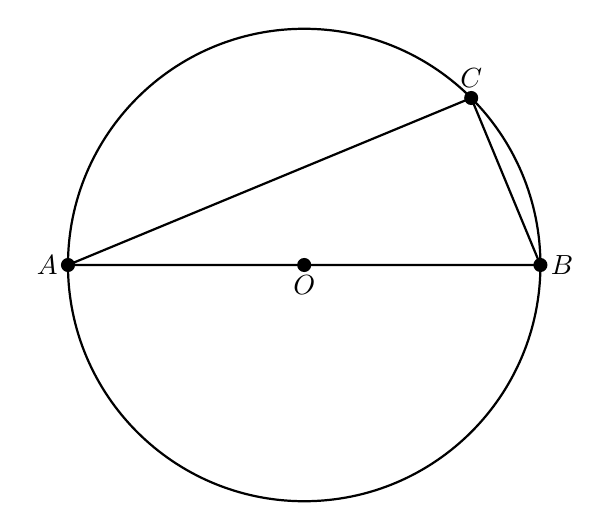
\begin{tikzpicture}[thick]
     \draw[fill=white] (0,0) circle (3);
\draw[-,thick](-3,0)--(3,0)--(.707*3,.707*3)--(-3,0);     
               \draw[fill=black] (0,0) circle (.75mm) node[below]{$O$};
                          \draw[fill=black] (-3,0) circle (.75mm) node[left]{$A$};
                                     \draw[fill=black] (3,0) circle (.75mm) node[right]{$B$};
                                                \draw[fill=black] (.707*3,.707*3) circle (.75mm) node[above]{$C$};
 
     
     
   \end{tikzpicture}
 \end{center}


\ifsat
	\begin{enumerate}[label=\Alph*)]
		\item   5 %
		\item  6
		\item  10
		\item  Cannot be determined.
	\end{enumerate}
\else
\fi

\ifacteven
	\begin{enumerate}[label=\textbf{\Alph*.},itemsep=\fill,align=left]
		\setcounter{enumii}{5}
		\item   5 %
		\item  6
		\item  10
		\addtocounter{enumii}{1}
		\item  12 
		\item  Cannot be determined.
	\end{enumerate}
\else
\fi

\ifactodd
	\begin{enumerate}[label=\textbf{\Alph*.},itemsep=\fill,align=left]
		\item   5 %
		\item  6
		\item  10
		\item  12 
		\item  Cannot be determined.
	\end{enumerate}
\else
\fi

\ifgridin
   5 %
		
\else
\fi

